\chapter{Aprendizaje automático y profundo}

	\section{Perceptrón}
	
		Ya en el año 1958, el psicólogo Frank Rosenblatt propuso un modelo llamado perceptrón el cual estaba basado en el comportamiento y funcionamiento de las neuronas de un humano, y que podía aprender ponderando cada coeficiente de entrada a la neurona\cite{historiaIA}. Hoy en día, tal y como se mostrará en esta sección, el perceptrón es la unidad fundamental de muchos modelos de \textit{machine learing} y \textit{deep learning}. \\
		
		Como se verá durante esta sección, este modelo ayuda a solucionar problemas de clasificación supervisada. Se dispone de una serie de valores de entrada $x_1, x_2, \hdots, x_n$ y se tiene una serie de valores de salida $y_1, y_2, \hdots, y_m$ que representan a qué clase pertenece la entrada ($2^m$ clases posibles). Esto se consigue mediante la ayuda de sus parámetros, que son una serie de pesos $w_1, w_2, \hdots, w_n$ y un sesgo o \textit{bias} $b$; y sus hiperparámetros, entre los que se encuentra una función $f$ de activación. 
		
		\begin{figure}[!h]
			\centering
			\begin{tikzpicture}
				\foreach \i in {1, 2}
					\pgfmathsetmacro{\resta}{int(\i - 1)}
					\node[circle, draw, fill=gray!20] (x-\i) at (0, -1 * \resta - \resta) {$x_{\i}$};
				\node (dots) at (0, -4) {$\vdots$};
				\node[circle, draw, fill=gray!20] (x-3) at (0, -6) {$x_{n}$};
				\node[circle, draw, fill=gray!20] (n) at (5,-3) {$n_1$};
				\node[circle, draw, fill=gray!20] (a) at (7,-3) {$a_1$};
				\node[circle, draw, fill=gray!20] (b) [below = of n] {$b_1$};
				\node[circle, draw, fill=gray!20] (y) [right = of a] {$y_1$};
				
				\foreach \i in {1, 2}
					\draw[-] (x-\i) -- (n) node [midway, above, sloped] {$w_{\i}$};
				\draw[-] (x-3) -- (n) node [midway, below, sloped] {$w_n$};
				\draw[-] (n) -- (a);
				\draw[-] (a) -- (y);
				\draw[-] (b) -- (n) node [midway, right] {$1$};
			\end{tikzpicture}
			\caption{Arquitectura de un perceptrón}
			\label{fig:perceptron}
		\end{figure}
		
		En la \Cref{fig:perceptron} se muestra la arquitectura del caso más simple de un perceptrón. Se tienen $n$ entradas y una única salida. La primera parte del diagrama representa que tal y como decía Rosenblatt, cada valor de entrada debe multiplicarse por un cierto peso, de tal forma que si se representa esto en función de sus valores en un instante $k$, lo que se computa en el nodo $n_1$ es la siguiente operación. 
		
		$$
		n_1(k) = b_1(k) + \sum_{i=1}^n x_i(k)w_i(k)
		$$
		
		Una vez se ha realizado este cálculo, el valor pasa por una función de activación en el nodo $a_1$, pues esta arquitectura es común utilizarla para clasificar una entrada y es muy útil obtener una salida binaria donde se active únicamente la salida que represente la clase a la que pertenece la entrada dada. Aunque existen diferentes funciones de activación para las neuronas, al trabajar con un perceptrón, la función de activación por excelencia es la función escalón de Heaviside, donde $\mathcal{U}: \mathbb{R} \longrightarrow \{0, 1\}$ y su expresión analítica es
		
		$$
		\mathcal{U}(x) = \left\{\begin{array}{ccc}
			0 & \text{si} & x < 0\\
			1 & \text{si} & x \geq 0
		\end{array}
		\right..
		$$
		
		Combinando ambas expresiones, se puede resumir en que la salida del perceptrón es equivalente a la siguiente ecuación: 
		
		$$
		y_1(k) = \left\{\begin{array}{ccc}
			0 & \text{si} & b_1(k) + \displaystyle\sum_{i=1}^n x_i(k)w_i(k) < 0\\
			1 & \text{si} & b_1(k) + \displaystyle\sum_{i=1}^n x_i(k)w_i(k) \geq 0
		\end{array}
		\right.
		$$
		
		Para dar un ejemplo claro de cómo funciona el perceptrón, se pueden tomar una serie de observaciones que tengan dos valores de entrada y uno de salida. Además, se supondrá que existen dos clases. Esto a fin de cuentas es asignar un valor de 0 o 1 a cada punto de $\mathbb{R}^2$ tal y como se describe en la \Cref{fig:labeled_data}. 
		
		\begin{figure}[!h]
			\centering
			\begin{tikzpicture}
				\begin{axis}[ymin = -2.5, ymax = 2.5, xmax = 2.5, xmin = -2.5, xticklabel = \empty, yticklabel = \empty, minor tick num = 1, axis lines = middle, xlabel = $x$, ylabel = $y$]
					\addplot[only marks, mark = *] coordinates {(1, 2)};
					\addplot[only marks, mark = triangle*] coordinates {(-1, 2) (0, -1)};
				\end{axis}
			\end{tikzpicture}
			\caption{Puntos etiquetados en $\mathbb{R}^2$}
			\label{fig:labeled_data}
		\end{figure}
		
		Una solución rápida sería trazar una recta $r: ax + by + c = 0$ que separe $\mathbb{R}^2$ en dos regiones, de forma que todo punto que pertenezca a una región pertenece entonces a una misma clase, tal y como se observa en la \Cref{fig:separated_label_data}. Esta recta suele llamarse \textit{decision boundary} o frontera de decisión. El problema entonces es hallar la recta $r$, pero se cumple que para este ejemplo es de la forma $w_1 x + w_2 y + b = 0$, siendo el problema encontrar los parámetros adecuados del modelo. La idea puede extrapolarse a diferente tamaño de entrada tomando un hiperplano de la forma $\textbf{w}^t \textbf{x} + b = 0$. \\
		
		Las preguntas a resolver ahora son, ¿existen siempre dichos parámetros? ¿Cómo pueden hallarse? El propio Minsky se hizo estas preguntas en \cite{perceptrons} y se dio cuenta de que dichos parámetros sí pueden hallarse en un número finito de pasos, siempre y cuando los puntos sean linealmente separables. Un ejemplo que no es linealmente separable es el de la función XOR tal y como se muestra en la \Cref{table:xor,fig:xor}, pues no existe una recta $r$ que separe $\mathbb{R}^2$ en dos regiones de tal forma que cada región contenga puntos de una única clase, sería necesaria una frontera de decisión no lineal. 
		
		\begin{figure}
			\centering
			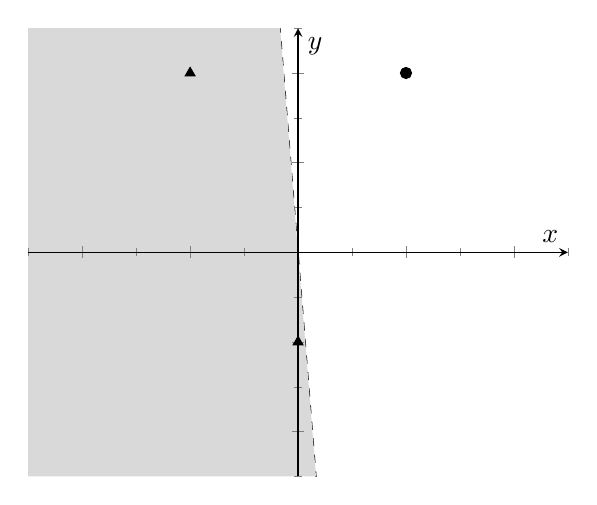
\begin{tikzpicture}
				\begin{axis}[ymin = -2.5, ymax = 2.5, xmax = 2.5, xmin = -2.5, xticklabel = \empty, yticklabel = \empty, minor tick num = 1, axis lines = middle, xlabel = $x$, ylabel = $y$, axis on top]
					\addplot[only marks, mark = *] coordinates {(1, 2)};
					\addplot[only marks, mark = triangle*] coordinates {(-1, 2) (0, -1)};
					\addplot[domain = -3:3, samples = 2, dashed] {-15*x};
					\draw[fill = gray!30, draw = none] (axis cs:-2.5, -2.5) -- (axis cs:-2.5, 2.5) -- (axis cs: -1/6, 2.5) -- (axis cs:1/6, -2.5);
				\end{axis}
			\end{tikzpicture}
			\caption{Puntos separados en $\mathbb{R}^2$}
			\label{fig:separated_label_data}
		\end{figure}
		
		\begin{table}[H]
			\centering
			\begin{tabular}{|c|c|c|}\hline
				$x$ & $y$ & $x \oplus y$\\\hline
				0 & 0 & 0\\\hline
				0 & 1 & 1\\\hline
				1 & 0 & 1\\\hline
				1 & 1 & 0\\\hline
			\end{tabular}
			\caption{Función XOR}
			\label{table:xor}
		\end{table}
		
		\begin{figure}
			\centering
			\begin{tikzpicture}
				\begin{axis}[ymin = -.5, ymax = 2.5, xmax = 2.5, xmin = -.5, xticklabel = \empty, yticklabel = \empty, minor tick num = 1, axis lines = middle, xlabel = $x$, ylabel = $y$]
					\addplot[only marks, mark = *] coordinates {(0, 0) (1, 1)};
					\addplot[only marks, mark = triangle*] coordinates {(0, 1) (1, 0)};
				\end{axis}
			\end{tikzpicture}
			\caption{Valores de $x \oplus y$ en  $\mathbb{R}^2$}
			\label{fig:xor}
		\end{figure}
		
		En cuanto a la pregunta de cómo hallar los parámetros, se consideran las siguientes ecuaciones\cite{nndesign}, donde $\textbf{w}$ es el vector de pesos, $t$ el valor esperado, y $a$ la salida del perceptrón y se aplica el \Cref{algo:perceptron} para obtener los parámetros óptimos. En dicho algoritmo se supondrá que existe una matriz $X$ de $n$ filas que contiene los diferentes $\textbf{x}$. 
		
		\begin{equation}
			\label{eq:perceptron}
			\begin{gathered}
				\textbf{w}(k+1) = \textbf{w}(k) + e(k)\textbf{x}(k)\\
				b(k+1) = b(k) + e(k)\\
				e(k) = t(k) - a(k)\\
				a(k) = \mathcal{U}(\textbf{w}^t(k)\textbf{x}(k))
			\end{gathered}
		\end{equation}
		
		
		\begin{algorithm}
			\SetProgSty{texttt}\DontPrintSemicolon
			
			\caption{Regla de aprendizaje del perceptrón}
			\label{algo:perceptron}
			
			\Datos{$X, \textbf{t}$}
			\Resultado{$\textbf{w}, b$}
			$b \gets 0$\\
			$\textbf{w} \gets$ \texttt{random}\\
			$k \gets 0$\\
			\Repetir{$\lnot$\texttt{acabar}}{
				\texttt{acabar} $\gets$ \texttt{true}\\
				\Para{$i \gets k$ \KwTo $k + n - 1$}{
					$e(i) \gets t(i) - a(i)$\\
					$\textbf{w}(i+1) \gets \textbf{w}(i) + e(i)\textbf{x}(i \pmod n)$\\
					$b(i+1) \gets b(i) + e(i)$\\
					\texttt{acabar} $\gets$ \texttt{acabar} $\land \, e(i) == 0$ 
				}
				$k \gets k + n - 1$
			}
		\end{algorithm}
		
		A cada una de las iteraciones que realiza el bucle exterior se les denomina épocas o \textit{epoch}, que consiste en realizar el proceso de entrenamiento sobre todo el conjunto de datos. En este caso se está suponiendo que no va a recibir casos que no sean linealmente separables, pero de lo contrario se puede añadir un contador \texttt{max\_epochs} y fijar un número máximo para no caer en un bucle infinito. No sería tarea fácil determinar dicho valor, pues aunque el algoritmo converge en los casos previamente explicados, no en todos lo hace de manera rápida. A continuación se muestra cómo obtener una solución para el caso de la \Cref{fig:labeled_data} aplicando el \Cref{algo:perceptron}. 
		
		$$
		X = \begin{pmatrix}
			1 & -1 & 0\\
			2 & 2 & -1
		\end{pmatrix} \,\,\, \textbf{t} = \begin{pmatrix}
		1 & 0 & 0
		\end{pmatrix} \,\,\, \textbf{w}(0) = \begin{pmatrix}
		1\\1 \end{pmatrix} \,\,\, b(0) = 0
		$$
		
		\begin{enumerate}[label = \textbf{\arabic*. }]
			\setcounter{enumi}{-1}
			\item \begin{itemize}
				\item $a(0) = \mathcal{U}(\textbf{w}^t(0)\textbf{x}(0)) = \mathcal{U}\left(\begin{pmatrix}1 & 1\end{pmatrix}\begin{pmatrix}
					1\\2 \end{pmatrix} + 0\right) = 1$
				\item $e(0) = t(0) - a(0) = 1 - 1 = 0$
				\item $\textbf{w}(1) = \textbf{w}(0)$
				\item $b(1) = b(0)$
			\end{itemize}
			
			\item \begin{itemize}
				\item $a(1) = \mathcal{U}(\textbf{w}^t(1)\textbf{x}(1)) = \mathcal{U}\left(\begin{pmatrix}1 & 1\end{pmatrix}\begin{pmatrix}
					-1\\2 \end{pmatrix} + 0\right) = 1$
				\item $e(1) = t(1) - a(1) = 0 - 1 = -1$
				\item $\textbf{w}(2) = \textbf{w}(1) + e(1)\textbf{x}(1) = \begin{pmatrix}1\\ 1\end{pmatrix} - \begin{pmatrix}-1\\2\end{pmatrix} = \begin{pmatrix}2\\ -1\end{pmatrix}$
				\item $b(2) = b(1) + e(1) = -1$
			\end{itemize}
			
			\item \begin{itemize}
				\item $a(2) = \mathcal{U}(\textbf{w}^t(2)\textbf{x}(2)) = \mathcal{U}\left(\begin{pmatrix}2 & -1\end{pmatrix}\begin{pmatrix}
					0\\-1 \end{pmatrix} -1\right) = 1$
				\item $e(2) = t(2) - a(2) = 0 - 1 = -1$
				\item $\textbf{w}(3) = \textbf{w}(2) + e(2)\textbf{x}(2) = \begin{pmatrix}2\\ -1\end{pmatrix} - \begin{pmatrix}0\\-1\end{pmatrix} = \begin{pmatrix}2\\ 0\end{pmatrix}$
				\item $b(3) = b(2) + e(2) = -2$
				\item $\texttt{acabar} = \texttt{true} \land \texttt{false} \land \texttt{false} = \texttt{false}$
			\end{itemize}
			
			\item \begin{itemize}
				\item $a(3) = \mathcal{U}(\textbf{w}^t(3)\textbf{x}(3\pmod{3})) = \mathcal{U}\left(\begin{pmatrix}2 & 0\end{pmatrix}\begin{pmatrix}
					1\\2 \end{pmatrix} -2\right) = 1$
				\item $e(3) = t(3) - a(3) = 1 - 1 = 0$
				\item $\textbf{w}(4) = \textbf{w}(3)$
				\item $b(4) = b(3)$
			\end{itemize}
			
			\item \begin{itemize}
				\item $a(4) = \mathcal{U}(\textbf{w}^t(4)\textbf{x}(4\pmod{3})) = \mathcal{U}\left(\begin{pmatrix}2 & 0\end{pmatrix}\begin{pmatrix}
					-1\\2 \end{pmatrix} -2\right) = 0$
				\item $e(4) = t(4) - a(4) = 0 - 0 = 0$
				\item $\textbf{w}(5) = \textbf{w}(4)$
				\item $b(5) = b(4)$
			\end{itemize}
			
			\item \begin{itemize}
				\item $a(5) = \mathcal{U}(\textbf{w}^t(5)\textbf{x}(5\pmod{3})) = \mathcal{U}\left(\begin{pmatrix}2 & 0\end{pmatrix}\begin{pmatrix}
					0\\-1 \end{pmatrix} -2\right) = 0$
				\item $e(5) = t(5) - a(5) = 0 - 0 = 0$
				\item $\textbf{w}(6) = \textbf{w}(5)$
				\item $b(6) = b(5)$
				\item $\texttt{acabar} = \texttt{true} \land \texttt{true} \land \texttt{true} = \texttt{true}$
			\end{itemize}
		\end{enumerate}
		
		La ejecución del algoritmo finaliza tras dos épocas, donde en la primera de ellas va ajustando los pesos y el sesgo de manera adecuada, y en la segunda verifica que todas las observaciones han sido clasificadas de manera correcta. La frontera de decisión obtenida es la recta $r: 2x - 2 = 0$, que es una recta vertical. Una observación a realizar es que $\textbf{x}(1) \in r$, por tanto ¿a qué clase pertenece? Esto depende de la función de activación empleada, al utilizar $\mathcal{U}$ la clasificación es correcta, pero al cambiarla por otra, podría no serlo y necesitaría de más épocas para realizar correctamente la clasificación. \\
		
		La última cuestión que queda por tratar respecto al perceptrón es el porqué se verifica que en el caso de que los puntos dados sean linealmente separables, en un número finito de pasos, el \Cref{algo:perceptron} terminará su ejecución y con el $\textbf{w}$ óptimo, tal y como se enunciaba en el \textbf{Teorema de Convergencia del Perceptrón}. A continuación se realiza su demostración basándose en la que se encuentra en \cite{nndesign} pero de forma más clara y simple. Para comenzar con la demostración será necesario definir una serie de elementos, comenzando por $\Omega(k)$ y $\textbf{z}(k)$. Se entiende que se están concatenando vectores, no definiendo ``vectores dentro de vectores''. 
		
		$$
		\Omega(k) = \begin{pmatrix}
			\textbf{w}(k)\\
			b(k)
		\end{pmatrix} \,\,\, \textbf{z}(k) = \begin{pmatrix}
		\textbf{x}(k)\\
		1
		\end{pmatrix}
		 \,\,\, \Omega(0) = \begin{pmatrix}
			0\\0\\\vdots\\0
		\end{pmatrix}
		$$
		
		Con estos elementos y el cálculo de $a(k)$ en la \Cref{eq:perceptron} es fácil ver que $n(k) = \Omega^t(k)\textbf{z}(k)$. Recordando los posibles valores de $t(k)$, se deseaba que si dicho valor era 1, entonces $n(k) \geq 0$; y en caso de que valiese 0 entonces se deseaba tener $n(k) < 0$, en resumen, que $t(k) - a(k) = 0$. Otra forma de ver esto es afirmar que en el caso en que $t(k) \neq a(k)$, entonces $\Omega(k)$ debe actualizarse de acuerdo a la \Cref{eq:perceptron}. De esta forma $\Omega(k + 1) = \Omega(k) + e(k)\textbf{z}(k)$. Ahora se considerará un vector $\Omega^*$ de forma que 
		$$
		\forall k \exists \Omega^* \,\, \mathcal{U}(\Omega^{*^t}\textbf{z}(k)) = t(k),
		$$
		es decir, $\Omega^*$ es el vector de pesos óptimo. Además, por comodidad se normalizarán todas las distancias del problema, de manera que $\|\Omega^{*}\| = 1$ y $\|\textbf{z}(k)\| \leq 1$. El último elemento a considerar será $\delta$, que será definido como
		$$
		\delta = \min\lbrace\Omega^{*^t}\textbf{z}(i)\rbrace, 
		$$
		tomando además que $\delta > 0$ pues otra manera de definirlo es la distancia al punto más cercano a la frontera de decisión óptima. Con estos elementos se puede comenzar la demostración. Como la regla de actualización es $\Omega(k + 1) = \Omega(k) + e(k)\textbf{z}(k)$, al vector de pesos en un determinado instante (clasificación fallida) se le suma o resta $\textbf{z}(k)$ y a priori no se sabe cuántas veces se va a repetir esto, por lo que la idea de la demostración será ver si la norma del vector de pesos tiene una cota superior e inferior, es decir, se para de sumar o restar otros vectores $\textbf{z}(i)$, de manera que el algoritmo terminaría. Para obtener esto basta con comparar el comportamiento de $\Omega^t(k) \Omega^*$ frente a $\Omega^t(k)\Omega(k)$ (es decir, $\|\Omega\|^2$). \\
		
		Con el primero de los términos, al tratar de corregir un error se verifica que
		
		$$
		\Omega^t(k+1)\Omega^* = (\Omega(k) + e(k)\textbf{z}(k))^t \Omega^* = \Omega^t(k)\Omega^* + e(k)\Omega^{*^t}\textbf{z}(k). 
		$$
		
		Además, por la manera en la que se ha definido $\delta$, el segundo sumando pertenece al intervalo $(-\infty, -\delta] \cup [\delta, \infty)$, pudiendo deducir la siguiente desigualdad, por lo que en una actualización el término sólo varía por lo menos en $\delta$ unidades.  
		
		\begin{equation}
			\label{eq:inf_delta}
			\Omega^t(k+1)\Omega^* \geq \Omega^t(k)\Omega^* + \delta
		\end{equation}
		
		De la misma manera que se ha analizado el comportamiento de $\Omega^t(k) \Omega^*$ se procede con la actualización de $\Omega^t(k)\Omega(k)$. 
		
		\begin{align*}
			\Omega^t(k+1)\Omega(k+1) &= (\Omega(k) + e(k)\textbf{z}(k))^t(\Omega(k) + e(k)\textbf{z}(k))\\
			&= \Omega^2(k) + (e(k)\textbf{z}(k))^2 + 2e(k)\Omega^t(k)\textbf{z}(k)\\
			&= \Omega^t(k)\Omega(k) + e^2(k)\textbf{z}^t(k)\textbf{z}(k) + 2e(k)\Omega^t(k)\textbf{z}(k)\\
			&= \Omega^t(k)\Omega(k) + e^2(k)\textbf{z}^t(k)\textbf{z}(k) + 2e(k)n(k)
		\end{align*}
		
		En el segundo sumando se tiene que siempre será menor o igual que 1, pues por definición $0 \leq \textbf{z}^t(k)\textbf{z}(k) = \|\textbf{z}(k)\|^2 \leq 1$. Además, el tercer sumando siempre será cero o negativo, pues en todos los casos posibles en los que $e(k) \neq 0$ se cumple que $e(k)n(k) < 0$: 
		
		\begin{itemize}
			\item Si $t(k) = 1 \land n(k) < 0$, entonces $a(k) = 0 \land e(k) > 0$
			\item Si $t(k) = 0 \land n(k) \geq 0$, entonces $a(k) = 1 \land e(k) < 0$
		\end{itemize}
		
		De esta situación se puede deducir la siguiente desigualdad, por lo que en una actualización el término sólo varía en como máximo una unidad.   
		
		\begin{equation}
			\label{eq:sup_delta}
			\Omega^t(k+1)\Omega(k+1) \leq \Omega^t(k)\Omega(k) + 1
		\end{equation}
		
		Una vez se ha observado cómo varían estos términos al actualizarlos, se puede observar qué pasaría con ellos al hacer $m$ actualizaciones. Con el resultado obtenido en las \Cref{eq:inf_delta,eq:sup_delta} se pueden deducir las desigualdades $\delta m \leq \Omega^t(m)\Omega^*$ y $\Omega^t(m)\Omega(m) \leq m$. \\
		
		Ahora al aplicar la desigualdad de Cauchy--Schwarz\footnote{Esta desigualdad afirma que $\|\textbf{u}\textbf{v}\| \leq \|\textbf{u}\|\|\textbf{v}\|$. }, el valor de $\|\Omega^*\|$, y la propiedad transitiva, se obtiene una cota superior y otra inferior (ambas recuadradas) para $\|\Omega^t(m)\|$, lo que demuestra que el número de actualizaciones es finito y que por tanto el algoritmo converge. 
		
		\begin{align*}
			\boxed{\delta m} &\leq \Omega^t(m)\Omega^* = \|\Omega^t(m)\Omega^*\|\\
			&\leq \|\Omega^t(m)\| \|\Omega^*\| = \|\Omega^t(m)\| = \sqrt{\Omega^t(m)\Omega(m)}\\
			& \leq \boxed{\sqrt{m}} 
		\end{align*}
		
		$$
		\pushQED{\qed} 
		\delta m \leq \|\Omega(m)\| \leq \sqrt{m} \,\,\, \Longrightarrow \,\,\, m \leq \frac{1}{\delta^2}\qedhere
		\popQED
		$$ 
		
		Esta última desigualdad muestra cómo existe una relación entre el número de iteraciones del algoritmo y la distancia de los datos de entrenamiento a la frontera de decisión óptima (depende únicamente de esto). Cuanto más cerca estén, mayor será el número de iteraciones necesarias. 
		
	\section{Funciones de activación}
	
		Durante el estudio del perceptrón, se muestra cómo se emplea la función de Heaviside como función de activación en la neurona. Esto se debe a que se busca una función que independientemente de los valores de entrada que reciba, produzca una salida binaria. En ciertos casos, no se deseará una salida binaria pues el problema no tendría porqué ser de clasificación. Además, como se mostrará en modelos de machine y deep learing en secciones sucesivas, será importante que dicha función sea derivable en todo su dominio, cosa que no cumple $\mathcal{U}(x)$, pues no es continua en $x=0$. Por estos motivos, se presentan las funciones de activación más conocidas e importantes\cite{funcionesActivacion}. 
		
		\begin{itemize}
			\item \textbf{Función lineal}
			
			\begin{figure}[!h]
				\centering
				\begin{tikzpicture}
					\draw[->] (-2,0) -- (2,0) node[right] {$x$};
					\draw[->] (0,-2) -- (0,2) node[above] {$f(x)$};
					
					\draw[domain = -2:2, smooth, variable = \x] plot ({\x},{\x});
					\node[right] at (1.5,2.5) {$f(x) = x$};
				\end{tikzpicture}
				\caption{Función lineal}
				\label{fig:funcion_lineal}
			\end{figure}
			
			Con motivo de emplear una función que no produzca valores binarios, se pueden tomar funciones lineales $f: \mathbb{R} \longrightarrow \mathbb{R}$ de la forma $f(x) = ax$. Como se verá al emplear redes neuronales, no es muy útil al trabajar con tareas complejas, solo es capaz de cumplir con su tarea en problemas sencillos. Como se estudiará en sucesivas secciones, esto en parte se debe a la expresión de su derivada. Al ser un polinomio, es continua y derivable en todo $\mathbb{R}$, teniendo que
			$$
			\frac{df}{dx} = a
			$$
			y en el caso en el que se tome $a = 1$, se tiene que
			$$
			\frac{df}{dx} = f(x). 
			$$
			
			\item \textbf{Función logística}
			
			\begin{figure}[!h]
				\centering
				\begin{tikzpicture}
					\begin{axis}[
						xlabel = $x$,
						ylabel = {$f(x)$},
						xmin = -10, xmax = 10,
						ymin = 0, ymax = 1,
						width = 0.8\textwidth,
						height = 0.35\textwidth,
						xticklabel = \empty,
						yticklabel = \empty,
						axis lines = middle,
						domain = -10:10,
						samples = 100,
						]
						\addplot[black] {1/(1 + exp(-x))};
						\node at (axis cs: 5,0.8) {$f(x) = \frac{1}{1 + e^{-x}}$};
					\end{axis}
				\end{tikzpicture}
				\caption{Función logística}
				\label{fig:funcion_sigmoide}
			\end{figure}
			
			Esta vez también se presenta una función que no devuelve valores binarios, es conocida como función sigmoide por la forma de S que tiene, y es una función $f: \mathbb{R} \longrightarrow (0, 1)$. Una propiedad que es muy útil es que 
			$$
			\frac{df}{dx} = f(x)(1 - f(x)). 
			$$
			
			Es un intento de mejora de la función de activación empleada en el perceptrón, pues una ligera variación en la entrada puede crear un gran cambio en la salida. Esta función evita que eso suceda, pues una pequeña variación en la entrada produce una variación pequeña en la salida. 
			
			\item \textbf{Tangente hiperbólica}
			\begin{figure}[!h]
				\centering
				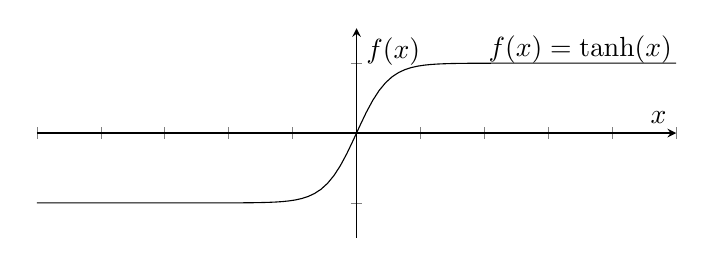
\begin{tikzpicture}
					\begin{axis}[
						xlabel = $x$,
						ylabel = {$f(x)$},
						xmin = -10, xmax = 10,
						ymin = -1.5, ymax = 1.5,
						width = 0.8\textwidth,
						height = 0.35\textwidth,
						xticklabel = \empty,
						yticklabel = \empty,
						axis lines = middle,
						domain = -10:10,
						samples = 100,
						]
						\addplot[black] {tanh(x)};
						\node at (axis cs: 7, 1.2) {$f(x) = \tanh(x)$};
					\end{axis}
				\end{tikzpicture}
				\caption{Tangente hiperbólica}
				\label{fig:funcion_tanh}
			\end{figure}
			
			De nuevo, se presenta una función que no devuelve valores binarios, y que guarda cierta relación con la logística, pues esta tiene también forma de sigmoide, pero a diferencia que la logística, esta verifica que $f(-x) = -f(x)$ por lo que es preferible sobre la logística, y también hace que al usarla en redes neuronales su entrenamiento converja más rápido. Además $f: \mathbb{R} \longrightarrow (-1, 1)$ y su expresión es
			$$
			f(x) = \tanh(x) = \frac{\text{senh}(x)}{\cosh(x)} = \frac{e^x - e^{-x}}{e^x + e^{-x}}, 
			$$
			verificando una segunda propiedad muy útil, 
			$$
			\frac{df}{dx} = 1 - f^2(x). 
			$$
			
			\item \textbf{Función ReLU}
			
			\begin{figure}[!h]
				\centering
				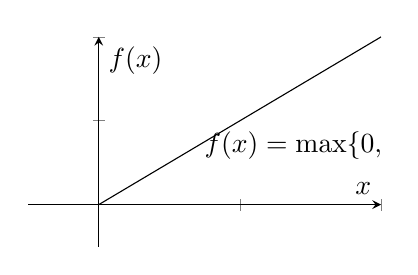
\begin{tikzpicture}
					\begin{axis}[
						xlabel = $x$,
						ylabel = {$f(x)$},
						xmin = -.5, xmax = 2,
						ymin = -.5, ymax = 2,
						width = 0.5\textwidth,
						height = 0.35\textwidth,
						xticklabel = \empty,
						yticklabel = \empty,
						axis lines = middle,
						domain = -.5:2,
						samples = 100,
						]
						\addplot[black, domain = 0:2] {x};
						\node at (axis cs: 1.5, .7) {$f(x) = \max\{0, x\}$};
					\end{axis}
				\end{tikzpicture}
				\caption{Función ReLU}
				\label{fig:funcion_relu}
			\end{figure}
			
			La función ReLU (Rectified Linear Unit) es una de las más populares al trabajar con redes neuronales, pues a pesar de que no es derivable en $x = 0$ (normalmente se soluciona tomando $f'(0) = 1$), soluciona un serio problema que causan las funciones logística y tangente hiperbólica durante el entrenamiento de una red neuronal. Este problema es conocido como \textit{vanishing gradient} y de forma resumida consiste en que cuando la derivada de una función es muy próxima a cero, relentiza enormemente el proceso de aprendizaje, pues si un determinado peso se actualiza de acuerdo a $$w_{ij}^{(m)}(k+1) = w_{ij}^{(m)}(k) - \alpha\frac{\partial e(k)}{\partial w_{ij}^{(m)}},$$ el segundo término será muy pequeño y se necesitarán muchas iteraciones para cambiar el valor del peso. Como se observa a continuación, la función ReLU soluciona este problema. Además, la derivada es mucho más sencilla de calcular. 
			
			\begin{align*}
				\lim_{x\to\infty}\frac{d}{dx}\frac{1}{1+e^{-x}} = 0 && \lim_{x\to\infty}\frac{d}{dx}\tanh(x) = 0 && \lim_{x\to\infty}\frac{d}{dx}\text{ReLU}(x) = 1
			\end{align*}
			
		\end{itemize}
		
	\section{Redes neuronales artificiales}
	
		El descubrimiento del perceptrón junto con el teorema que garantizaba que cualquier conjunto de puntos linealmente separable podría ser aprendido mediante este, supuso un gran avance en la IA al igual que una gran desilusión por parte de muchos al no poder aprender una función tan simple como la XOR. Esto causó el llamado el primer invierno de la IA, que finalizó con la llegada de las redes neuronales multicapa y el algoritmo de la retroprogragación. \\
		
		En 1989, George Cybenko enunció y consiguió demostrar el \textbf{Teorema de Aproximación Universal}\cite{teoremaAproximacion}. Este afirma que dada una red neuronal con una capa de entrada, una capa oculta con suficientes neuronas, y una capa de salida; es un aproximador universal de funciones. Es decir, si existe una relación entre dos variables $\textbf{x}$ e $\textbf{y}$, entonces una red neuronal con la arquitectura mencionada y el entrenamiento adecuado, encontrará dicha relación y podrá comportarse como una función $f$ tal que $\textbf{y} = f(\textbf{x})$. Este se considera un gran resultado, pues consigue acabar con las limitaciones del perceptrón que habían generado un decaimiento por el interés en la IA. 
		
		\begin{figure}[!h]
			\centering
			\begin{tikzpicture}
				\node[circle, draw, fill=gray!20] (x-1) {$x_{1}$};
				\foreach \i in {2,3}{
					\pgfmathtruncatemacro{\resta}{\i - 1}
					\node[circle, draw, fill=gray!20, below = of x-\resta] (x-\i) {$x_{\i}$};
				}
				\node (dots) [below = of x-3] {$\vdots$};
				\foreach \i in {1,2,3}{
					\node[circle, draw, fill=gray!20, right = 2cm of x-\i] (a-\i) {$a^{(1)}_{\i}$};
				}
				\node (dots2) [below = of a-3] {$\vdots$};
				\node (a-4) [circle, draw, fill=gray!20, below = of dots2] {$a^{(1)}_m$};
				\foreach \i in {1,2,3}{
					\node[circle, draw, fill=gray!20, right = 2cm of a-\i] (A-\i) {$a^{(s)}_{\i}$};
				}
				\node (dots3) [below = of A-3] {$\vdots$};
				\node (x-4) [circle, draw, fill=gray!20, left = 2cm of a-4] {$x_n$};
				\node (A-4) [circle, draw, fill=gray!20, below = of dots3] {$a^{(s)}_p$};
				\foreach \i in {1,2,3,4}{
					\node [left = .6cm of A-\i] {$\cdots$};
					\foreach \j in {1,2,3,4}{
						\draw[-] (x-\i) -- (a-\j);
					}
				}
				\foreach \i in {1,2,3}{
					\node (y-\i) [circle, draw, fill=gray!20, right =  of A-\i] {$y_{\i}$};
					\draw[-] (A-\i) -- (y-\i);
				}
				\node (y-4) [circle, draw, fill=gray!20, right =  of A-4] {$y_{p}$};
				\draw[-] (A-4) -- (y-4);
				\node (dots4) [right = 1.6cm of dots3] {$\vdots$};
			\end{tikzpicture}
			\caption{Arquitectura de una red neuronal multicapa}
			\label{fig:rna}
		\end{figure}
		
		En la \Cref{fig:rna} se muestra un diagrama que resume la arquitectura de una red neuronal multicapa. Todas las salidas de una capa están conectadas con todas las entradas de la siguiente con un peso y un \textit{bias}. En el diagrama de la \Cref{fig:rna_completa} se puede observar esto en mayor detalle. Estas pueden ser utilizadas en problemas de clasificación o regresión supervisada, pero en una primera aproximación se supondrá que se está resolviendo un problema de regresión. 
		
		\begin{figure}[!h]
			\centering
			\resizebox{\textwidth}{!}{
				\begin{tikzpicture}
					\node[circle, draw, fill=gray!20] at (4, 0) (n-1) {$n^{(1)}_{1}$};
					\node[circle, draw, fill=gray!20, below= .5cm of n-1] (b-1) {$b^{(1)}_{1}$};
					\foreach \i in {2,3}{
						\pgfmathtruncatemacro{\resta}{\i - 1}
						\node[circle, draw, fill=gray!20, below= 2 cm of b-\resta] (n-\i) {$n^{(1)}_{\i}$};
						\node[circle, draw, fill=gray!20, below= .5cm of n-\i] (b-\i) {$b^{(1)}_{\i}$};
					}
					\node[circle, draw, fill=gray!20, below left = 2 cm and 7 cm of n-1] (x-1) {$x_{1}$};
					\foreach \i in {2,3}{
						\pgfmathtruncatemacro{\resta}{\i - 1}
						\node[circle, draw, fill=gray!20, below= 2cm of x-\resta] (x-\i) {$x_{\i}$};
					}
					\node (dots) [below = .5cm of x-3] {$\vdots$};
					\node[circle, draw, fill=gray!20, below = .5cm of dots] (x-n) {$x_{n}$};
					\node (dots2) [below = .5cm of b-3] {$\vdots$};
					\node[circle, draw, fill=gray!20, below= .5cm of dots2] (n-n) {$n^{(1)}_{m}$};
					\node[circle, draw, fill=gray!20, below= .5cm of n-n] (b-n) {$b^{(1)}_{m}$};
					\foreach \i in {1,2,3}{
						\draw[-] (n-\i) -- (b-\i) node [midway, right] {$1$};
					}
					\draw[-] (b-n) -- (n-n) node [midway, right] {$1$};
					\foreach \i in {1,2,3}{
						\foreach \j in {1,2,3}{
							\pgfmathtruncatemacro{\condicion}{ifthenelse(Mod(\i, 2)==0,1,0)}
							\ifnum\condicion=1
							\draw[-] (x-\i) -- (n-\j) node [near start, above, sloped] {$w^{(1)}_{\j\i}$};
							\else
							\draw[-] (x-\i) -- (n-\j) node [near end, above, sloped] {$w^{(1)}_{\j\i}$};
							\fi
						}
					}
					\foreach \i in {1,2,3}{
						\draw[-] (x-n) -- (n-\i) node [near start, above, sloped] {$w^{(1)}_{\i n}$};
						\draw[-] (x-\i) -- (n-n) node [near end, below, sloped] {$w^{(1)}_{m\i}$};
					}
					\draw[-] (x-n) -- (n-n) node [midway, below, sloped] {$w^{(1)}_{mn}$};
					\foreach \i in {1,2,3}{
						\node[circle, draw, fill=gray!20, right = 1cm of n-\i] (a-\i) {$a^{(1)}_{\i}$};
					}
					\node[circle, draw, fill=gray!20, right = 1cm of n-n] (a-n) {$a^{(1)}_{m}$};
					\foreach \i in {1,2,3}{
						\draw[-] (n-\i) -- (a-\i);
					}
					\draw[-] (n-n) -- (a-n);
					\foreach \i in {1,2,3}{
						\node [right = .7cm of a-\i] {$\cdots$};
						\node[circle, draw, fill=gray!20, right = 2cm of a-\i] (N-\i) {$n^{(s)}_{\i}$};
					}
					\node[circle, draw, fill=gray!20, right = 2cm of a-n] (N-4) {$n^{(s)}_{p}$};
					\node [right = .7cm of a-n] {$\cdots$};
					\foreach \i in {1,2,3}{
						\node[circle, draw, fill=gray!20, right = 1cm of N-\i] (A-\i) {$a^{(s)}_{\i}$};
					}
					\node[circle, draw, fill=gray!20, right = 1cm of N-4] (A-4) {$a^{(s)}_{p}$};
					\foreach \i in {1,2,3,4}{
						\draw[-] (N-\i) -- (A-\i);
					}
					\foreach \i in {1,2,3}{
						\node[circle, draw, fill=gray!20, below= .5cm of N-\i] (B-\i) {$b^{(s)}_{\i}$};
						\draw[-] (N-\i) -- (B-\i) node [midway, right] {$1$};
					}
					\node [below = .5cm of B-3] {$\vdots$};
					\node[circle, draw, fill=gray!20, below= .5cm of N-4] (B-4) {$b^{(s)}_{p}$};
					\draw[-] (N-4) -- (B-4) node [midway, right] {$1$};
					\foreach \i in {1,2,3}{
						\node[circle, draw, fill=gray!20, right = 22 cm of x-\i] (y-\i) {$y_{\i}$};
					}
					\node[circle, draw, fill=gray!20, right = 22 cm of x-n] (y-4) {$y_{p}$};
					\foreach \i in {1,2,3,4}{
						\draw[-] (A-\i) -- (y-\i);
					}
				\end{tikzpicture}
			}
			\caption{Red neuronal multicapa}
			\label{fig:rna_completa}
		\end{figure}
		
		Al igual que un perceptrón quedaba representado mediante un vector $\textbf{w}$ de pesos y un valor de sesgo $b$, para representar una red neuronal multicapa se hace mediante las matrices $W^{(m)}$ y los vectores $\textbf{b}^{(m)}$ y $\textbf{f}^{(m)}$, que contienen los pesos, los sesgos, y las funciones de activación. La notación para los sesgos es $b_i^{(m)}$, que representa el sesgo de la entrada $i-$ésima de la capa $m$. De igual manera $f_i^{(m)}$ representa la función de activación la neuona $i-$ésima de la capa $m$. Para los pesos, $w_{ij}^{(m)}$ denota el peso que une la salida $j$ con la entrada $i$ de la capa $m$. Para las capas, $1 \leq m < M$. En ningún momento un exponente entre paréntesis representa una potencia, en dicho caso aparecerá sin paréntesis para distinguirlo. Siguiendo los mismos pasos que con el perceptrón, la primera pregunta será cómo calcular la salida de una red neuronal. La salida de una capa se calcula con la \Cref{eq:prop}, teniendo en cuenta que $\textbf{x}^{(m)} = \textbf{y}^{(m-1)}$, por lo que para calcular la salida de la red no hay más que aplicar dicha ecuación hasta llegar a la última capa. 
		
		\begin{equation}
			\label{eq:prop}
			\begin{gathered}
				\textbf{a}^{(m)}(k) = F^{(m)}\left(W^{(m)}(k)\textbf{x}^{(m)}(k) + \textbf{b}^{(m)}(k)\right)\\
				\begin{pmatrix}
					a_1^{(m)}(k)\\a_2^{(m)}(k)\\\vdots\\a_j^{(m)}(k)
				\end{pmatrix} = F^{(m)}\left(
				\begin{pmatrix}
					w_{11}^{(m)}(k) & w_{12}^{(m)}(k) & \cdots & w_{1i}^{(m)}(k)\\
					w_{21}^{(m)}(k) & w_{22}^{(m)}(k) & \cdots & w_{2i}^{(m)}(k)\\
					\vdots & \vdots & \ddots & \vdots\\
					w_{j1}^{(m)}(k) & w_{j2}^{(m)}(k) & \cdots & w_{ji}^{(m)}(k)\\
				\end{pmatrix}
				\begin{pmatrix}
					x_1^{(m)}(k)\\x_2^{(m)}(k)\\\vdots\\x_i^{(m)}(k)
				\end{pmatrix} + 
				\begin{pmatrix}
					b_1^{(m)}(k)\\b_2^{(m)}(k)\\\vdots\\b_j^{(m)}(k)
				\end{pmatrix}\right)
			\end{gathered}
		\end{equation}
		
		A continuación, se puede plantear cuál es la ecuación del error para una red neuronal. Esta es simplemente cuestión de elección al igual que las funciones de activación. Al trabajar con redes neuronales para problemas de regresión, la función de error por excelencia es el error cuadrático, definido como
		$$
		L(k) = \sum(\textbf{t}(k) - \textbf{a}^{(M)}(k))^2, 
		$$
		aunque existen otras muchas, cada una adecuada a cada tipo de problema y modelo, como por ejemplo el error cuadrático medio, error absoluto, error absoluto medio, error logarítmico, error exponencial, entropía cruzada, etc\cite{funcionesError}.\\
		
		La pregunta ahora sería que, al igual que existía una ecuación para actualizar los parámetros del perceptrón ¿existe para una red neuronal? Para deducirla fácilmente, basta en pensar que $L$ es una función que depende de los parámetros de la red y que se quiere que su valor sea lo más pequeño posible para diferentes vectores de entrada, es decir, encontrar los valores de los parámetros que minimizan $L$. Esto es un problema clásico de cálculo que en el caso de una variable se resuelve igualando a cero la derivada de la función, y en el caso de varias, mediante la matriz Hessiana. Sin embargo, dichos métodos para una función de tantas variables y con expresiones complejas, no son muy eficientes. \\
		
		Esto se soluciona con ayuda de un algoritmo conocido como descenso por gradiente\cite{descenso}. Este algoritmo calcula de manera iterativa una aproximación de los mínimos de una función con ayuda del vector gradiente de una función. El vector gradiente de una función $f$ se define como 
		$$
		\nabla f(x_1, x_2, \hdots, x_n) = \left(\frac{\partial f}{\partial x_1}, \frac{\partial f}{\partial x_2}, \hdots, \frac{\partial f}{\partial x_n}\right), 
		$$
		e indica la dirección en la que la función crece más rápido, siendo la idea principal del algoritmo ir moviéndose en dirección contraria a este. 
		
		\begin{algorithm}
			\SetProgSty{texttt}\DontPrintSemicolon
			
			\caption{Descenso por gradiente}
			\label{algo:descenso}
			
			\Datos{$f, \alpha, k$}
			\Resultado{$\textbf{x}(k)$}
			$\textbf{x}(0) \gets$\texttt{ random}\\
			\Para{$i \gets 1$ \KwTo $k$}{
				$\textbf{x}(i + 1) = \textbf{x}(i) - \alpha\nabla f(\textbf{x}(i))$
			}
		\end{algorithm}
		
		Como se observa en el \Cref{algo:descenso}, se comienza en un punto aleatorio, lo que puede variar la calidad de la solución dependiendo de la ejecución, y además se introduce un término $\alpha$ llamado \textbf{tasa de aprendizaje}. Pueden existir casos en los que la magnitud del gradiente sea muy grande, lo que resulta en desplazamientos bruscos y una convergencia más lenta, tal y como se refleja en la \Cref{fig:descenso}. Si se hubiese fijado un valor máximo de $k = 25$, en los casos de las \Cref{fig:descenso_grande,fig:descenso_peq}, no se hubiese llegado a una buena aproximación del mínimo por haber elegido un $\alpha$ inadecuado. 
		
		\begin{figure}[!h]
			\centering
			\begin{subfigure}{.3\textwidth}
				\centering
				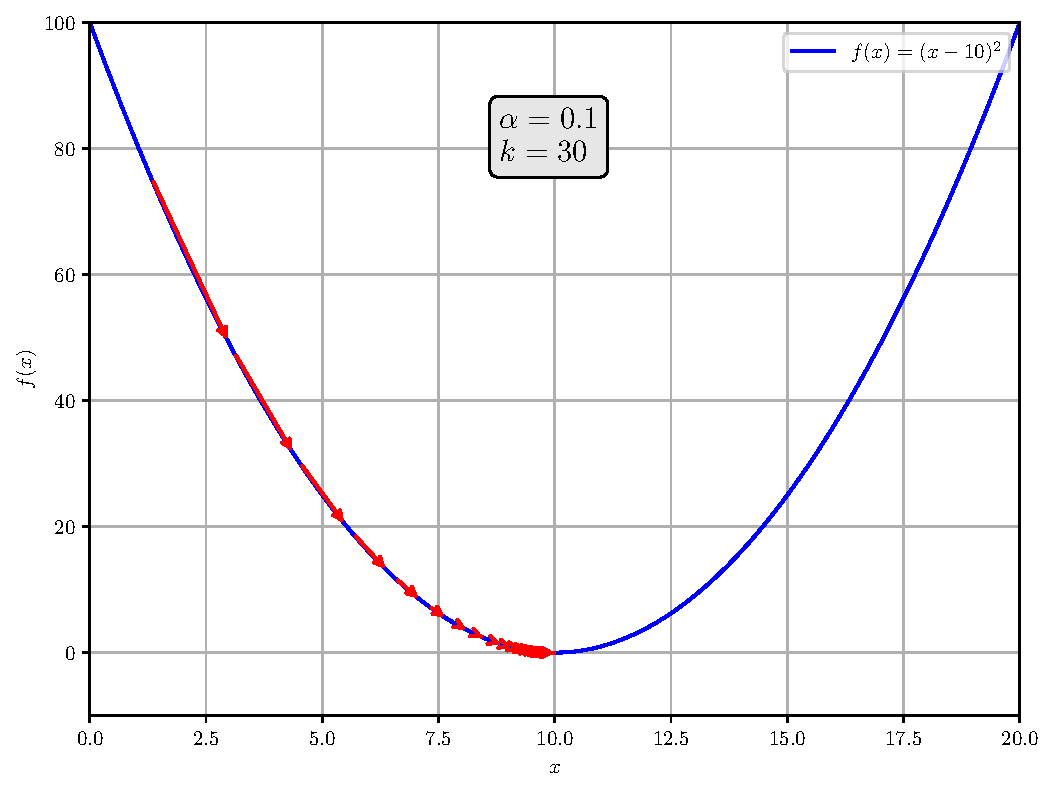
\includegraphics[width = \linewidth]{descenso}
				\caption{$\alpha$ adecuada}
			\end{subfigure}
			\begin{subfigure}{.3\textwidth}
				\centering
				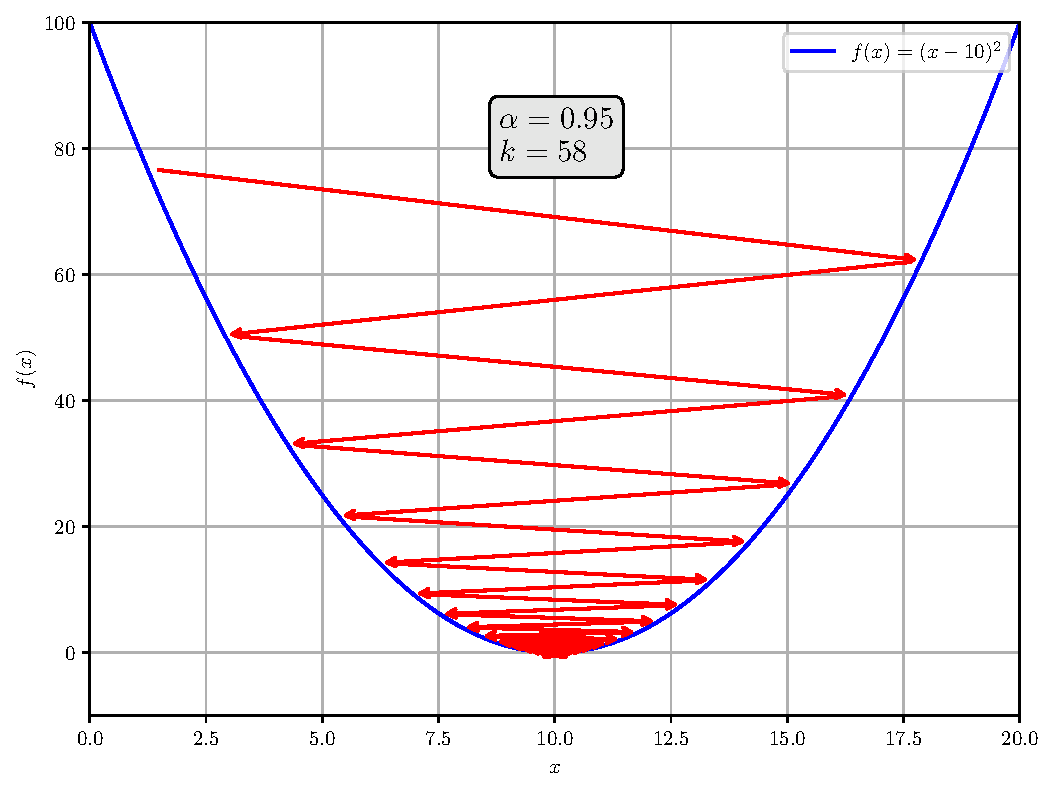
\includegraphics[width = \linewidth]{descenso2}
				\caption{$\alpha$ demasiado grande}
				\label{fig:descenso_grande}
			\end{subfigure}
			\begin{subfigure}{.3\textwidth}
				\centering
				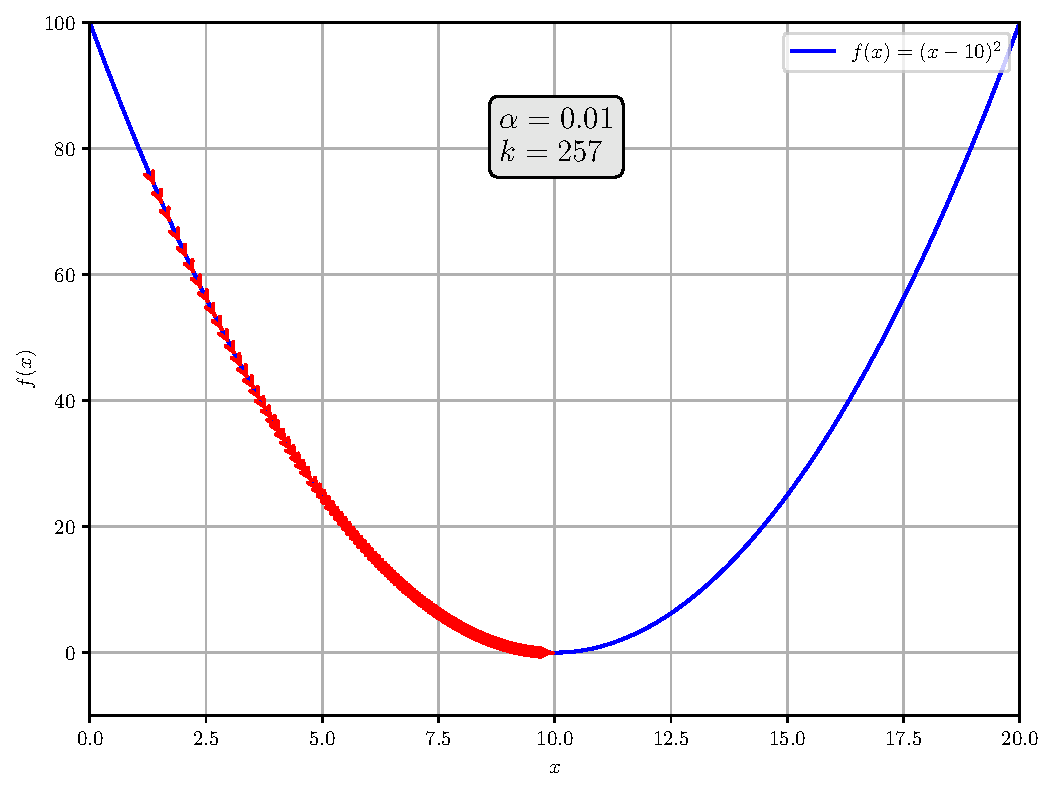
\includegraphics[width = \linewidth]{descenso3}
				\caption{$\alpha$ demasiado pequeña}
				\label{fig:descenso_peq}
			\end{subfigure}
			\caption{Descenso por gradiente}
			\label{fig:descenso}
		\end{figure}
		
		Con esta idea de la función de error y el descenso por gradiente, aparece el famoso algoritmo de la retropropagación o \textit{backpropagation}. Es muy similar al algoritmo de aprendizaje del perceptrón pero adaptado a la estructura de una red neuronal. El primer paso consiste en dada una entrada, calcular la salida de la red con ayuda de la \Cref{eq:prop}. El segundo paso es calcular el error $L(k)$. Esta función depende de todos los pesos y sesgos de la red, por lo que el tercer paso será modificar estos de acuerdo a $\nabla L$ y repetir el procedimiento para el resto de observaciones. Se realizan tantas épocas como sean necesarias. \\
		
		El problema que queda por resolver es cómo calcular todos los elementos de $\nabla L$, pues por ejemplo es fácil calcular $\frac{\partial L}{\partial a_i^{(M)}}$, pero no parece tan obvio calcular $\frac{\partial L}{\partial w_{ij}^{(m)}}$, pues hay que retroceder $M-m$ capas, y habrá muchos valores que dependan de ese peso. La solución a esto es la regla de la cadena. 
		
		$$
		\frac{\partial f}{\partial x} = \frac{\partial f}{\partial u_1}\frac{\partial u_1}{\partial x} + \frac{\partial f}{\partial u_2}\frac{\partial u_2}{\partial x} + \hdots + \frac{\partial f}{\partial u_n}\frac{\partial u_n}{\partial x}
		$$
		
		Con ayuda de esta regla se pueden calcular fácilmente los términos no triviales del gradiente, propagando el error hacia atrás por la red hasta llegar al parámetro deseado mediante las sensibilidades $\left(\delta_i^{(s)}\right)$\cite{nndesign}. De aquí se intuye el porqué del nombre del algoritmo. De manera informal, lo que hace el algoritmo es castigar a cada neurona de manera proporcional a su participación en el error final. 
		
		$$
		\begin{gathered}
			\frac{\partial L}{\partial b_{i}^{(s)}} = \frac{\partial L}{\partial a_{i}^{(s)}} \frac{\partial a_{i}^{(s)}}{\partial n_{i}^{(s)}} \frac{\partial n_{i}^{(s)}}{\partial b_{i}^{(s)}} = \delta_i^{(s)}\\
			\frac{\partial L}{\partial w_{ij}^{(s)}} = \frac{\partial L}{\partial a_{i}^{(s)}} \frac{\partial a_{i}^{(s)}}{\partial n_{i}^{(s)}} \frac{\partial n_{i}^{(s)}}{\partial w_{ij}^{(s)}} = \delta_i^{(s)} \frac{\partial n_{i}^{(s)}}{\partial w_{ij}^{(s)}} = \delta_i^{(s)} a_j^{(s-1)}\\
			\delta_i^{(M)} = \frac{\partial L}{\partial a_{i}^{(M)}} \frac{\partial a_{i}^{(M)}}{\partial n_{i}^{(M)}} = -2a_{i}^{(M)} \frac{\partial a_{i}^{(M)}}{\partial n_{i}^{(M)}} = -2a_{i}^{(M)} \frac{\partial f_{i}^{(M)}}{\partial n_{i}^{(M)}}\\
			\delta_i^{(m)} = \frac{\partial L}{\partial n_i^{(m)}} = \sum_{l=1}^p\frac{\partial L}{\partial n_l^{(m+1)}}\frac{\partial n_l^{(m+1)}}{\partial n_i^{(m)}} = \sum_{l=1}^p \delta_l^{(m+1)} \frac{\partial n_l^{(m+1)}}{\partial n_i^{(m)}} = \sum_{l=1}^p \delta_l^{(m+1)} w_{li}^{(m+1)} \frac{\partial f_i^{(m)}}{\partial n_i^{(m)}}\\
			\text{con } 0 < m < M \text{ y } 0 < s \leq M
		\end{gathered}
		$$
		
		Estas ecuaciones pueden reescribirse de manera matricial para aligerar la notación, que combinándolas con las ideas explicadas referentes al \Cref{algo:descenso}, da lugar al \Cref{algo:backprop}, bastante similar al \Cref{algo:perceptron} pero adaptado a una red neuronal. 
		
		\begin{algorithm}
			\SetProgSty{texttt}\DontPrintSemicolon
			
			\caption{Retropropagación (\textit{backpropagation})}
			\label{algo:backprop}
			
			\Datos{}
			\Resultado{}
		\end{algorithm}
		
		